\section{Progress}
\label{sec:progress}

\subsection{RISC-V processor}
Setting up and running the vivado-risk-v \cite{vivado-risk-v} required the use of an Ubuntu 20.04 LTS environment to prevent issues with incorrect package versions being installed. The rocket64b1 core was generated successfully and the SD card was set up with a Linux environment. The \texttt{mk-sd-card} program required all partitions to be deleted from the SD card before use. The built-in flash function did not work so the Vivado GUI was used to manually program the FPGA through the hardware manager. This is only temporary and must be re-done every time the board is powered down but is sufficient for this project. Storing the bitstream on the SD card and loading it into the FPGA when powered could be investigated in the future. This used 77\% of the FPGAs LUTs limiting the space available for custom hardware (Figure \ref{fig:LUT_usage}).

\begin{figure}[h]
	\centering
	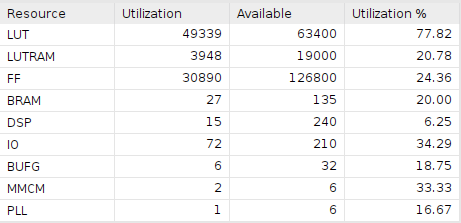
\includegraphics[scale=0.6]{../common/vivado-risk-v Uilization.png}
	\caption{Vivado utilisation report for risc-v processor}
	\label{fig:LUT_usage}
\end{figure}

Putty was used to connect the to RISC-V processors serial port with a baud rate of 115200. It displayed the Linux boot sequence showing the process was successful. Unfortunately, this boot process was extremely slow due to an issue with the udev daemon hindering development with it. There are also issues installing programs with \texttt{apt} in the Linux environment.

Due to the boot issue with Linux, bare-metal code proved to be a much better solution. The example hello-world bare-metal code from the vivado-risc-v project was successfully run to test the use of bare-metal code (Figure \ref{fig:helloworld}).

\begin{figure}[H]
	\centering
	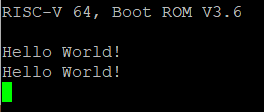
\includegraphics[scale=1]{bare-metal.png}
	\caption{Bare-metal "hello world" Script Serial Output}
	\label{fig:helloworld}
\end{figure}

\subsection{Adding IP}
The Vivado development environment provides a block view of the project. The AXI interface can be found in the IO block and custom IP blocks can be connected to this to make them available over AXI. To test this pre-made AXI GPIO block \cite{xilinx_gpio} was added and connected to a new master AXI connection on the \texttt{io\_axi\_s} block. The \texttt{axi\_clk} and \texttt{axi\_reset} lines were used for the new IPs clk and reset ports (Figure \ref{fig:gpio_ip}). The output of the GPIO block was connected to the FPGA board LEDs. Under the address editor, a new base address can be assigned to the GPIO block (Figure \ref{fig:address_editor}).

\begin{figure}[H]
	\centering
	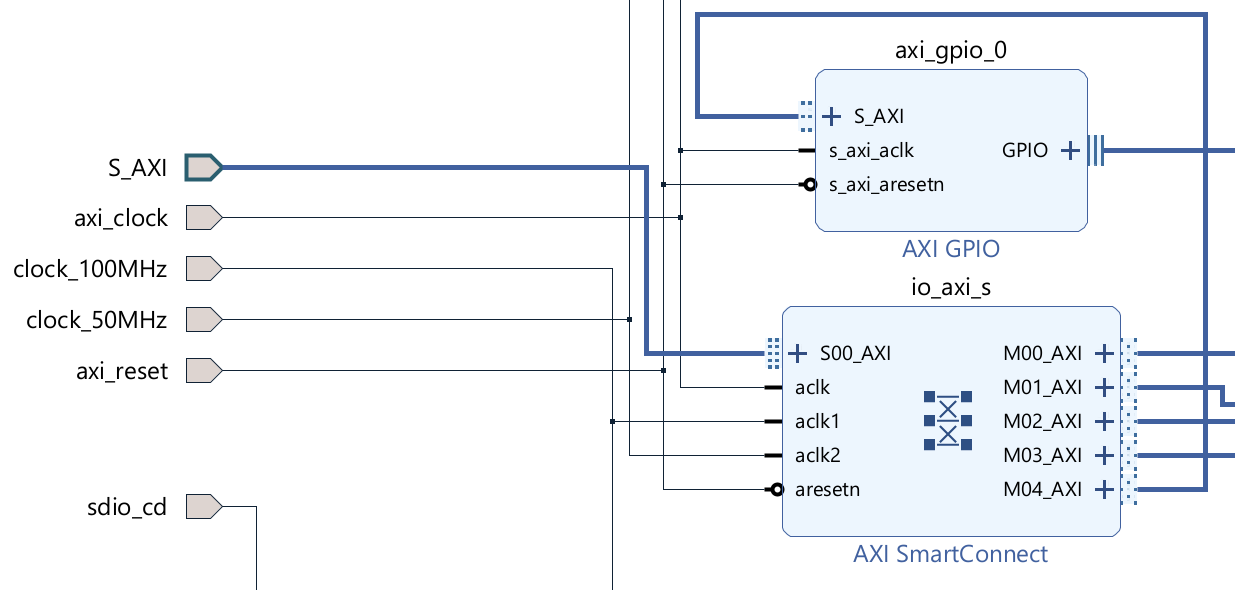
\includegraphics[scale=0.4]{GPIO_IP.png}
	\caption{Vivado IP Block Diagram}
	\label{fig:gpio_ip}
\end{figure}

\begin{figure}[H]
	\centering
	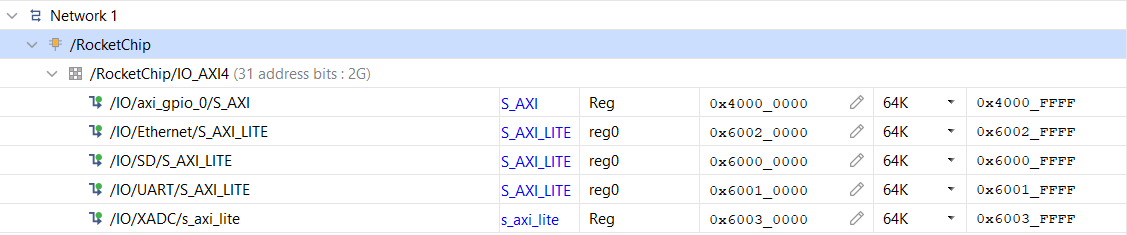
\includegraphics[scale=0.6]{address_editor.png}
	\caption{Vivado Address Editor}
	\label{fig:address_editor}
\end{figure}

Adding this to the device tree in the Linux environment using the example entry was unsuccessful and bare-metal code will be used this was not pursued further. Xilinx provides drivers \cite{xilinx_gpio_driver} for their built-in IP blocks but these are significantly more complicated due to the wide range of devices it must support and include libraries that are not available. The process for interfacing with the IP block is relatively simple. Four 32-bit memory registers start at the assigned base address which represents the data and direction for each of the two 32-bit channels made available. These can be set by writing a uint32 value to a pointer at an address offset from the specified base address. This can be simplified by using a struct (Listing \ref{lst:gpio-struct}).

The example hello-world code was used as a base for developing a script to test this and interact with the serial bus.

\begin{figure}[h]
\begin{lstlisting}[style=CStyle, caption={Definition of a structure to access virtual memory addresses.}, label={lst:gpio-struct}]
typedef struct gpio {
	volatile uint32_t gpio_data;  // Data reg 1
	volatile uint32_t gpio_tri;   // I/O direction reg 1
	volatile uint32_t gpio_data2; // Data reg 2
	volatile uint32_t gpio_tri2;  // I/O direction reg 2
} GPIO;

GPIO * gpio_reg = (GPIO *)base_address;
\end{lstlisting}
\end{figure}

\subsection{Custom AXI IP block}
When creating custom IP blocks in Vivado, a blank block can be generated or a block with a pre-made AXI interface \cite{xilinx_axiip}). To test the use of a custom IP block the pre-made AXI interface was used and custom Verilog code was added to it. This allowed data to be written to one register copied to a second one in hardware and then read back from the new register. A basic shift register was implemented to test processing the data before output but this is not yet working.

\section{Timeline}
The timeline for this project has changed considerably from the specification. It was initially planned to develop the hardware accelerator first and then integrate it into the RISC-V processor. However, it was decided that starting with the processor and building on that was better as the accelerator depends on the system of communication and that depends on the processor. The updated timeline (Table \ref{tab:timeline}) shows this change.

\begin{table}[H]
	\centering
	\resizebox{\textwidth}{!}{
		\begin{tabular}{|c|l|}
			\hline
			\multicolumn{1}{|l|}{Week} & Task                                                               \\ \hline
			2                          & Write specification                                                \\ \hline
			4                          & Generate a working RISC-V processor                                \\ \hline
			6                          & Integrate an IP block into the processors AXI bus                  \\ \hline
			8                          & Integrate a basic custom IP block into the processors AXI bus      \\ \hline
			10                         & Write the progress report                                          \\ \hhline{|=|=|}
			14                         & Develop a custom AXI interface IP block and driver code            \\ \hline
			16                         & Research and design the structure of the hardware accelerator      \\ \hline
			20                         & Implement accelerator in a custom IP block using the AXI interface \\ \hline
			21                         & Design and develop a performance test for the accelerator          \\ \hline
			23/24                      & Write presentation                                                 \\ \hline
			30                         & Write progress report                                              \\ \hline
		\end{tabular}
	}
	\caption{Updated timeline}
	\label{tab:timeline}
\end{table}

The next thing to be developed is a custom AXI interface. This may be based on the code provided by Xilinx or documentation from the developer of ZipCPU \cite{axi_lite_custom}. This will be used to interface with the accelerator by transmitting 32-bit values between the bare-metal code and the hardware. This has been assigned 4 weeks due to it going through the winter holiday.

Next research will be made into methods of building the hardware accelerator and a block design will be made to show how it will be structured before beginning development. Different methods should be considered to find what is best for this project. The designed accelerator can then be implemented in Verilog and connect to the AXI interface block. A bare-metal code driver will pass in the input data and validate the output. This will be used to test the functionality of the accelerator. Input data is currently planned to be stored directly in the code but if time is available it may be modified to allow data to be loaded from the SD card.

A performance test can then be developed and run using hardware and software approaches. This can then be compared to assess the usefulness of the accelerator.

Finally, the presentation and final report can be written.